\textbf{Primer parcial}
\begin{itemize}
%%Teoría propiedades, estática y blalances integrales
%% Propiedades y definiciones
\item ¿Cuál es la definición del concepto ``volumen de control''?
\item Las fuerzas externas pueden actuar sobre un volumen de control de dos maneras, ¿cuáles?
%% Hidrostática
\item ¿Cuál es la forma integral de la fuerza que una distribución de presiones $p(\vec{r})$ ejerce sobre una superficie $S$?
\item Escribir en forma vectorial el teorema general de la hidrostática. ¿Bajo qué hipótesis se cumple?
%% Balances integrales
\item ¿En qué principio físico se basa el balance integral de energía?
\item ¿En qué situación es nula la variación de masa dentro de un volumen de control?
%%--------------------------------------------------------
%%Ejercicios hidrostática
%%Tanques solidarios
\item Dos tanques que contienen dos fluidos diferentes se hallan separados por
una compuerta cuadrada, abisagrada en "A", como se muestra en la figura (\ref{fig:tanques}).
Cada uno de los tanques se ve sometido a una presión manométrica distinta en su
parte superior. ¿Cuál es la fuerza que debería aplicarse sobre la arista "B" para que la misma se mantenga cerrada?
\begin{center}
  $\rho_1 = 1100 \frac{kg}{m^3} \qquad P_{1,man} = -10 kPa \qquad H_1 = 10 m $\\
  $\rho_2 = 900 \frac{kg}{m^3} \qquad P_{2,man} = 50 kPa \qquad H_2 = 4 m$
\end{center}
\begin{figure}[h!!!!]
  \centering
  \includegraphics[width=0.4\textwidth]{tanques_solidarios.png}
  \caption{Tanques solidarios}
  \label{fig:tanques}
\end{figure}
%%Compuerta semiesférica
\item Calcular la fuerza aplicada por el fluido sobre la compuerta semiesférica representada en el esquema (\ref{fig:esfera}), sabiendo que se trata de agua a temperatura ambiente. La compuerta tiene un radio $R=1.5m$ y su  centroide se encuentra a una profundidad $H=4m$. Indique ambas componentes ($x$ e $y$) y el punto de aplicación de la fuerza.
  \begin{figure}[!!h]
    \centering
    \includegraphics[width=0.4\textwidth]{compuertaEsferica.png}
    \label{fig:esfera}
    \caption{Compuerta semiesférica sumergida}
  \end{figure}

%%Camion cisterna
\item El camión tanque semi remolque de la figura \ref{fig:remolque} pasa de $0$ a $20$ $m/s$, acelerando uniformemente durante $40s$. Se encuentra lleno de combustible ($\gamma=0,8$) hasta la mitad de su altura $A = 4$m. Las dimensiones restantes del contenedor son $B = 4$m y $L = 10$m. Calcular la fuerza que debe soportar la tapa trasera si la cisterna est\'a abierta y se encuentra dividida en \textbf{5 compartimientos}. A su vez, calcular qué aceleración del camión provoca el derrame de combustible.
  \begin{figure}[!ht]
    \centering
    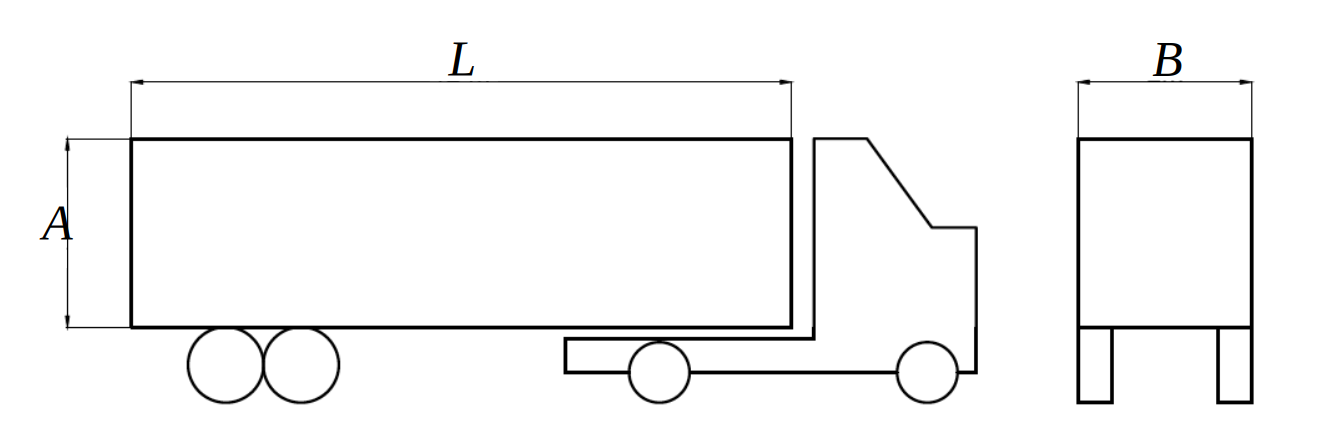
\includegraphics[width=0.8\textwidth]{camionCisterna.png}
    \caption{Esquema del camión cisterna}
    \label{fig:remolque}
  \end{figure}

%%Tanque rotante
 \item Calcular la velocidad de rotación máxima a la que puede girar el recipiente de la figura (\ref{fig:tacho}) sin que se derrame el líquido contenido en su interior. Calcular la presión sobre los puntos A y B para la velocidad de rotación calculada en el punto anterior. Los datos son los siguientes
  \begin{center}
    $\gamma = 800\frac{kgf}{m^3} \qquad H_m = 1.0 m \qquad h_0 = 0.6 m\qquad R = 0.5 m$
  \end{center}
  \begin{figure}[h!!]
    \centering
    \includegraphics[width=0.4\textwidth]{tacho.png}
    \caption{Recipiente cilíndrico en rotación}
    \label{fig:tacho}
  \end{figure}

%%Ejercicios Balances integrales
%%Codo Cimbala
\item Por el codo de la figura (\ref{fig:codo}) circulan $Q=1000 m^3/h$ de agua, con presión de entrada de $P_1 = 1.5 kg/cm^2$, siendo la pérdida de carga del mismo  de $\Delta h = 1.0m$. Calcular fuerza ejercida por el agua, considerando el codo emplazado en el plano horizontal (peso en el eje y). Los diámetros de la tubería son que $d_1 = 40$cm y $d_2 = 30$cm, $\theta = 30$. 
      \vspace{0.5cm}
      \begin{figure}[h!!]
      \centering
      \includegraphics[width=0.5\textwidth]{codo_cimbala_gral.png}
      \caption{Cálculo de fuerza en codo}
      \label{fig:codo}
      \end{figure}  
      
      
%% Codo 90°
\item Por el codo de la figura (\ref{fig:codo}) circulan $Q=1500 m^3/h$ de agua, con presión de entrada de \\ $P_1 = 6 kg/cm^2$, siendo la pérdida de carga del mismo  de $\Delta h = 1.0m$. Calcular fuerza ejercida por el agua, considerando el codo emplazado en el plano horizontal. Desprecie el peso del accesorio y del agua. Los diámetros de la tubería son que $d_1=30$cm y $d_2=20$cm
  \vspace{0.5cm}
  \begin{figure}[h!!]
  \centering
   \includegraphics[width=0.5\textwidth]{codo.pdf}
  \caption{Cálculo de fuerza en codo}
  \label{fig:codo}
  \end{figure}  

%%Codo deflector móvil
\item El accesorio cuya geometría se describe en la figura (\ref{fig:codoDeflector}) se desplaza hacia la derecha con una velocidad $\vec{U} = (2.5,\;0,\;0)$m/s. Calcular la fuerza y potencia ejercida por el fluido sobre la pieza en función de los siguientes parámetros:
\begin{center}
$\rho = 1000 \frac{kg}{m^3} \qquad
\vec{V}^{abs}_1 = (8.5,\;0,\;0) \frac{m}{s} \qquad P_{1,man} = 50000 Pa
\qquad A_1 = 0.1 m^2 \qquad A_2 = 0.05 m^2$
\end{center}

\begin{figure}[h!!]
\centering
\includegraphics[width=0.4\textwidth]{codoDeflector.png}
\caption{Codo deflector, Cengel Cimbala (capítulo 6)}
\label{fig:codoDeflector}
\end{figure}

\end{itemize}
